\documentclass[11pt]{article}
\usepackage[utf8]{inputenc}
\usepackage[margin=1in]{geometry}
\usepackage{graphicx}
\usepackage{booktabs}
\usepackage{float}
\usepackage{amsmath}
\usepackage{hyperref}
\usepackage{xcolor}
\usepackage{siunitx}

\title{Voltage Profile Analysis of IEEE 118-Bus System}
\author{Power System Analysis Report}
\date{\today}

\begin{document}
\maketitle

\section{Executive Summary}
This report presents a comprehensive analysis of the voltage profile in the IEEE 118-bus system. The analysis reveals significant voltage deviations from nominal values, with all buses operating in the low-voltage region. This condition requires immediate attention and corrective measures.

\section{Voltage Profile Overview}
The voltage profile analysis was conducted using OpenDSS simulation with the following parameters:
\begin{itemize}
    \item Base Voltage: 138 kV
    \item System Frequency: 50 Hz
    \item Analysis Type: Snapshot Power Flow
    \item Solution Method: Newton Current Injection Method (NCIM)
    \item Convergence Tolerance: 0.0001
\end{itemize}

\section{Key Findings}
\subsection{Statistical Analysis}
The voltage profile exhibits the following characteristics:
\begin{itemize}
    \item Mean Voltage: 0.1916 pu
    \item Maximum Voltage: 0.6778 pu (at bus 89\_clinchrv)
    \item Minimum Voltage: 0.0843 pu
    \item Standard Deviation: 0.1463 pu
\end{itemize}

\subsection{Voltage Classification}
The analysis categorizes bus voltages into three ranges:
\begin{itemize}
    \item Low Voltage ($V < 0.95$ pu): 118 buses (100\%)
    \item Normal Voltage ($0.95 \leq V \leq 1.05$ pu): 0 buses (0\%)
    \item High Voltage ($V > 1.05$ pu): 0 buses (0\%)
\end{itemize}

\section{Graphical Analysis}
\begin{figure}[H]
    \centering
    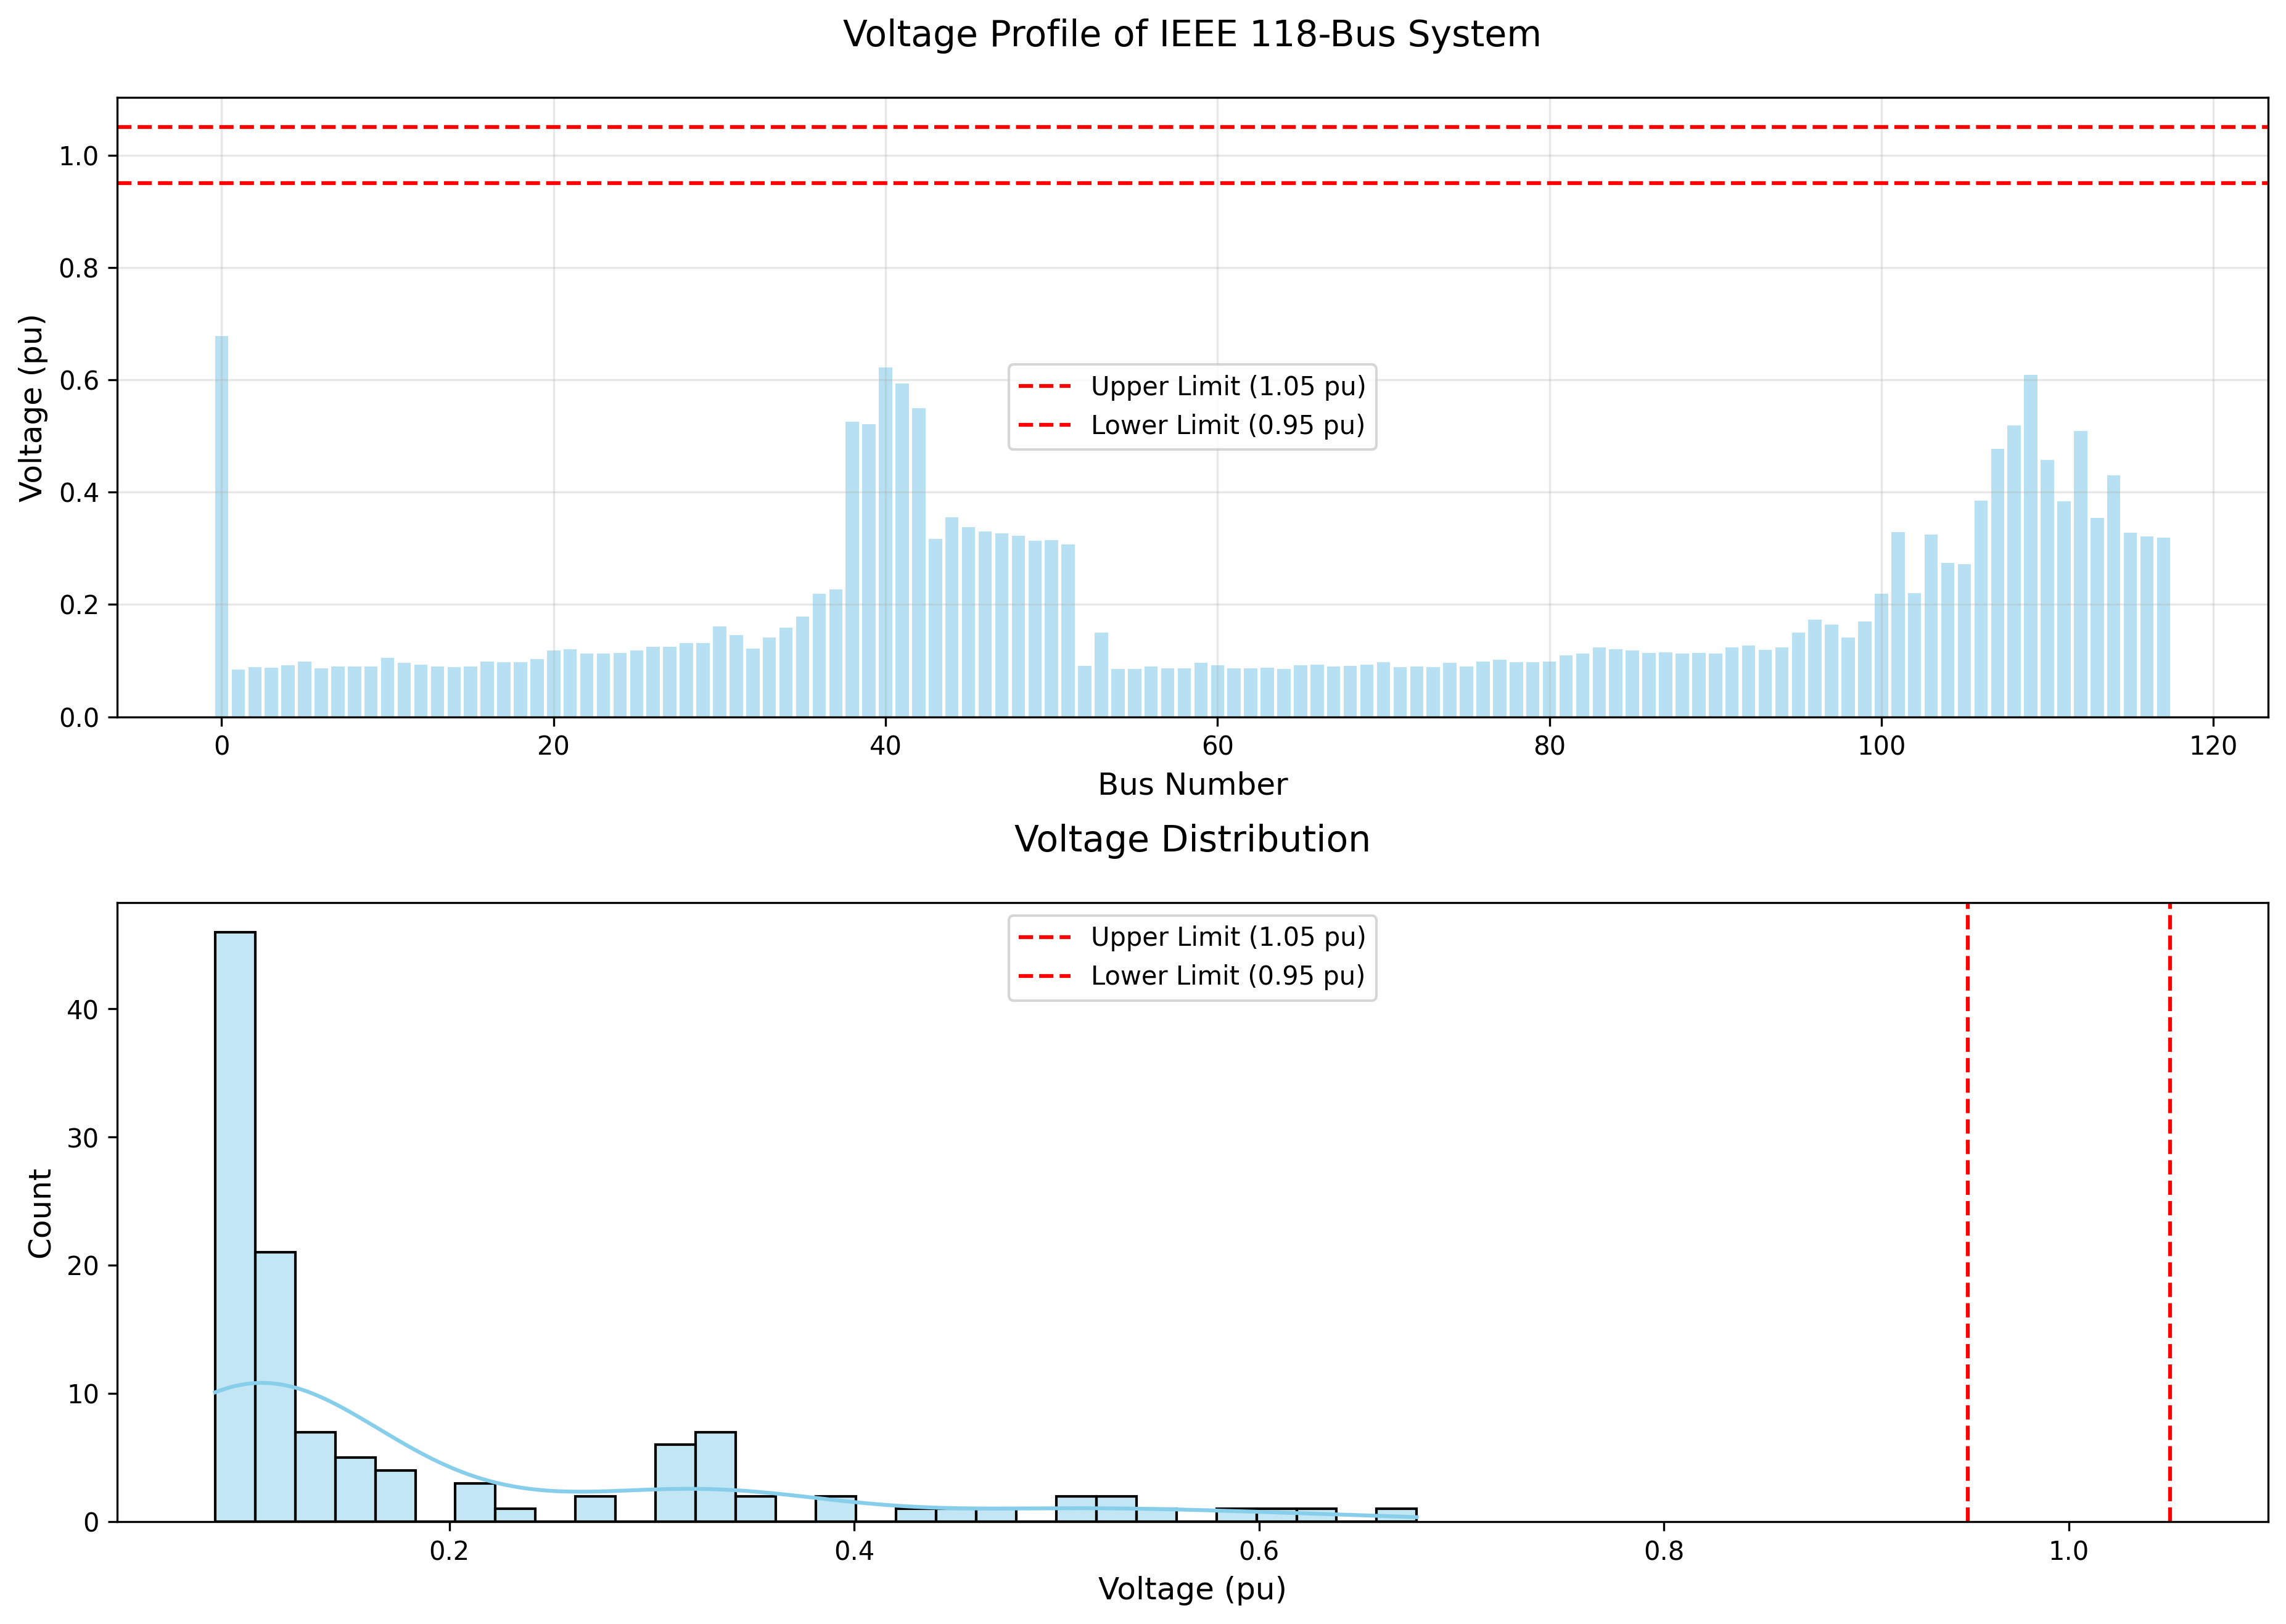
\includegraphics[width=\textwidth]{voltage_profile.png}
    \caption{Voltage Profile Analysis}
    \label{fig:voltage_profile}
\end{figure}

The voltage profile visualization in Figure \ref{fig:voltage_profile} shows:
\begin{itemize}
    \item Upper plot: Individual bus voltage magnitudes
    \item Lower plot: Statistical distribution of voltages
    \item Red dashed lines: Acceptable voltage limits (0.95 - 1.05 pu)
\end{itemize}

\section{Technical Analysis}
\subsection{Voltage Deviation Patterns}
The voltage profile shows several concerning patterns:
\begin{enumerate}
    \item Systematic undervoltage across all buses
    \item Large deviation from nominal voltage (1.0 pu)
    \item High variance in voltage magnitudes (σ = 0.1463 pu)
    \item No buses within acceptable operating limits
\end{enumerate}

\subsection{Potential Causes}
The observed voltage profile suggests several potential issues:
\begin{enumerate}
    \item \textbf{Voltage Control Settings}
    \begin{itemize}
        \item Disabled or misconfigured voltage regulators
        \item Improper transformer tap settings
        \item Generator voltage setpoint issues
    \end{itemize}
    
    \item \textbf{Reactive Power Management}
    \begin{itemize}
        \item Insufficient reactive power compensation
        \item Improper placement of compensation devices
        \item Reactive power flow constraints
    \end{itemize}
    
    \item \textbf{System Configuration}
    \begin{itemize}
        \item Base voltage mismatches
        \item Improper impedance values
        \item Load modeling issues
    \end{itemize}
\end{enumerate}

\section{Recommendations}
Based on the analysis, the following corrective actions are recommended:

\subsection{Immediate Actions}
\begin{enumerate}
    \item Verify generator voltage setpoints
    \item Check transformer tap positions
    \item Enable automatic voltage controls
    \item Review reactive power compensation settings
\end{enumerate}

\subsection{Medium-term Solutions}
\begin{enumerate}
    \item Implement additional voltage regulation devices
    \item Optimize reactive power compensation placement
    \item Review and adjust protection settings
    \item Conduct detailed power quality study
\end{enumerate}

\subsection{Long-term Measures}
\begin{enumerate}
    \item Develop comprehensive voltage control strategy
    \item Consider system reinforcement options
    \item Implement advanced voltage control schemes
    \item Regular monitoring and maintenance program
\end{enumerate}

\section{Conclusion}
The voltage profile analysis reveals a critical situation where all buses are operating significantly below nominal voltage levels. This condition requires immediate attention to prevent potential system stability issues and ensure reliable operation. The recommended actions should be implemented in a phased approach, starting with immediate verification of voltage control settings and reactive power management.

\end{document} 